\documentclass[../sparc.tex]{subfiles}
\graphicspath{{\subfix{../images/}}}
\begin{document}

%%%%%%%%%%%%%%%%%%%%%%%%%%%%%%%%%%%%%%%%%%%%%%%%%%%%%%%%%%%%%%%%%%%%%%%%%%%%%%%%
\section{Виды сигналов}

Существуют два основных вида сигналов -- \emph{аналоговые} и \emph{цифровые}.
Для их сравнения посмотрим на графики \ref{fig:adc-analog-signal-example} и
\ref{fig:adc-digital-signal-example}.

\begin{figure}[ht]
  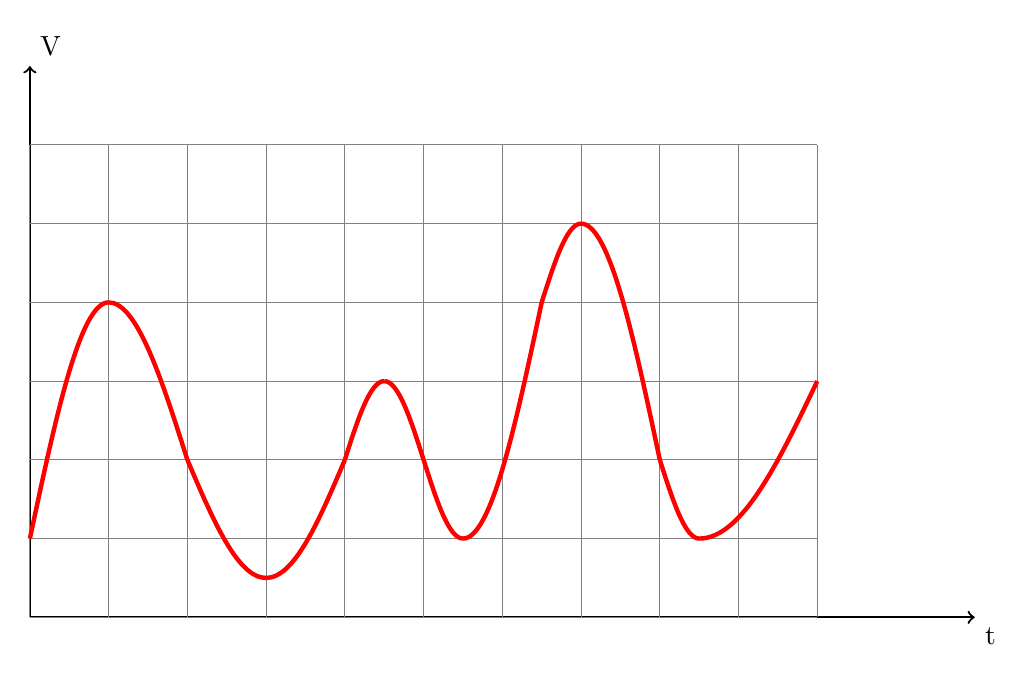
\begin{tikzpicture}
    \draw[thick, ->] (0, 0) -- (12, 0) node[anchor=north west] {t};
    \draw[thick, ->] (0, 0) -- (0,  7) node[anchor=south west] {V};
    \draw[gray] (0, 0) grid (10, 6);
    \draw[ultra thick, red] (0,1)   sin (1,4);
    \draw[ultra thick, red] (1,4)   cos (2,2);
    \draw[ultra thick, red] (2,2)   sin (3,0.5);
    \draw[ultra thick, red] (3,0.5) cos (4,2);
    \draw[ultra thick, red] (4,2)   sin (4.5,3);
    \draw[ultra thick, red] (4.5,3) cos (5,2);
    \draw[ultra thick, red] (5,2)   sin (5.5,1);
    \draw[ultra thick, red] (5.5,1) cos (6.5,4);
    \draw[ultra thick, red] (6.5,4) sin (7,5);
    \draw[ultra thick, red] (7,5)   cos (8,2);
    \draw[ultra thick, red] (8,2)   sin (8.5,1);
    \draw[ultra thick, red] (8.5,1) cos (10, 3);
  \end{tikzpicture}
  \caption{Пример аналогового сигнала.}
  \label{fig:adc-analog-signal-example}
\end{figure}

\begin{figure}[ht]
  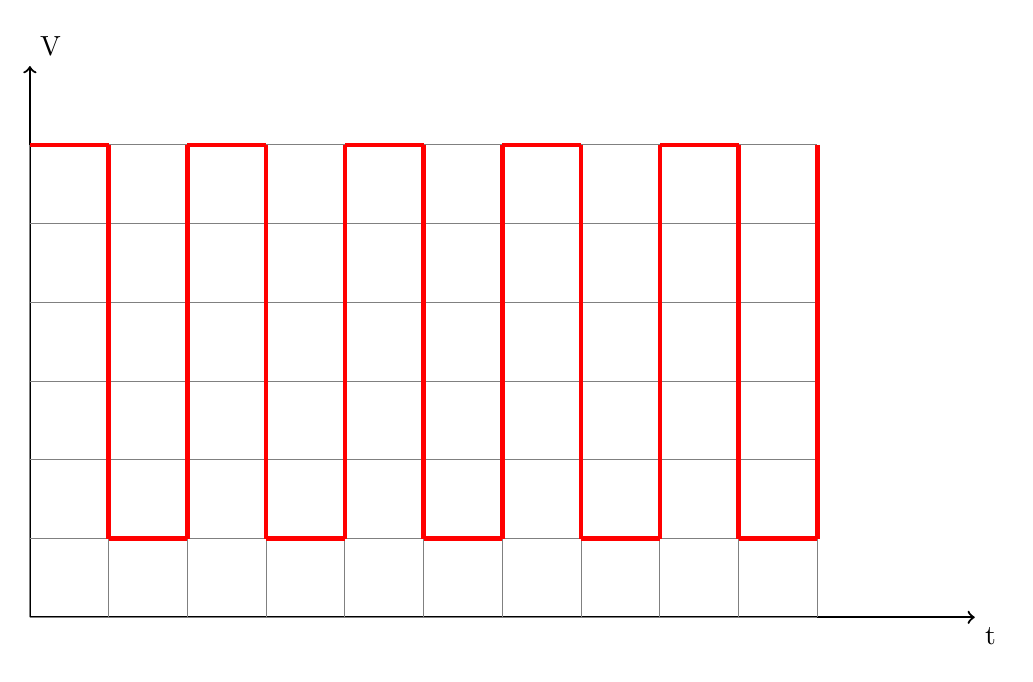
\begin{tikzpicture}
    \draw[thick, ->] (0, 0) -- (12, 0) node[anchor=north west] {t};
    \draw[thick, ->] (0, 0) -- (0,  7) node[anchor=south west] {V};
    \draw[gray] (0, 0) grid (10, 6);
    \foreach \x in {0, 2, ..., 8} {
      \draw[ultra thick, red] (\x, 6) -- (\x + 1, 6);
      \draw[ultra thick, red] (\x + 1, 6) -- (\x + 1, 1);
      \draw[ultra thick, red] (\x + 1, 1) -- (\x + 2, 1);
      \draw[ultra thick, red] (\x + 2, 1) -- (\x + 2, 6);
    }
  \end{tikzpicture}
  \caption{Пример цифрового сигнала.}
  \label{fig:adc-digital-signal-example}
\end{figure}

По оси ``Y'' на обоих графиках отложены Вольты, по оси ``X'' -- время.

Как можно видеть, аналоговый сигнал не имеет чётко выделенных уровней и меняется
произвольно во времени в некоторых пределах.  Цифровой сигнал имеет чётко
выраженные логические уровни, соответствующие нулю и единице.

Примером аналоговых сигналов является голос человека.  Если мы попробуем
записать голос на цифровой диктофон, то на микрофон диктофона будет приходить
звуковая волна, подобная той, что на рисунке
\ref{fig:adc-analog-signal-example}.

Примером цифрового сигнала является записанный звуковой файл, передаваемый по
сети Internet.  Если сохранить цифровой сигнал на накопитель, то получатся
цифровые данные, состоящие из нулей и единиц -- на обычных компьютерах подобные
данные, как правило, хранятся в виде файлов.

Также компьютеры обладают возможностью принимать и \emph{оцифровывать}
аналоговые сигналы.

Благодаря возможности считывать аналоговые сигналы, компьютер или
микроконтроллер может получать самую различную информацию об окружающем мире,
ведь масса различных параметров окружающей среды представлены именно некоторым
диапазоном значений, которые не имеют чётких делений: температура, влажность,
освещённость, атмосферное давление и т.п.

Именно поэтому большинство микроконтроллеров имеют аналоговые входы для работы с
аналоговыми сигналами, и в последующих разделах мы рассмотрим эти возможности на
примере платформы Arduino.

Но для начала мы должны изучить инструменты, которые позволят там видеть сигнал,
который приниммает и обрабатывает микроконтроллер.

\end{document}
